\chapter{Results \& Discussion}

\section{Software}
\subsection{PlantCV}
For our experiment’s preprocessing, We used PlantCV, an open-source Python library built on OpenCV and Matplotlib, because PlantCV offers modular functions for common plant phenotyping workflows. The abstractions provided by this library allows us to quickly implement and evaluate our image processing pipelines, and classification mechanisms. Furthermore, the paper’s code is extensible, and our results are more reproducible because PlantCV is open-source. Also, many contributors continuously optimize for modern hardware, so the use of this open-source software is more economical and performant than developing custom solutions from scratch.

\subsection{Scikit-image}
A forked and modified version of the open-source scikit-image library was used for feature extraction. This library is used to calculate the gray-level co-occurrence matrix (GLCM) from a grayscale image. However, the original implementation in this library did not allow the background to be excluded from its calculation, therefore, then texture from leaves and their background would be considered. Practically, this means that our feature vectors would not truly represent features of leaves, and therefore possibly lead to poor leaf disease detection performance.

\subsection{Scikit-learn}
The scikit-learn library was used to train, calculate, and evaluate metrics for the proposed SVM model.

\subsection{Study Code}
The code for this research can be found at the following GitHub repository \url{https://github.com/Darshan-Pillay/Honours-Research-Project}.

\section{Hardware}
Model training and preprocessing were performed on a 14-inch MAcBook Pro (2021) running macOS Sonoma 14.7.2, with an M1 Pro chip and 16 GB of RAM.

\section{Dataset}

\subsection{Plant Village}
The dataset used in this study is PlantVillage. It was previously available from the official PlantVillage website; however it is no longer accessible. So, we obtained a copy of the original dataset from \url{https://github.com/spMohanty/PlantVillage-Dataset}. This dataset contains images of various plant species’ leaves, including potato, pepper and tomato. For our experiment, we used a subset of PlantVillage, which includes 16,011 images comprising both healthy and diseased tomato leaves. These images were preprocessed to generate feature vectors for training our SVM model.

\begin{figure}[htbp]
	\centering
	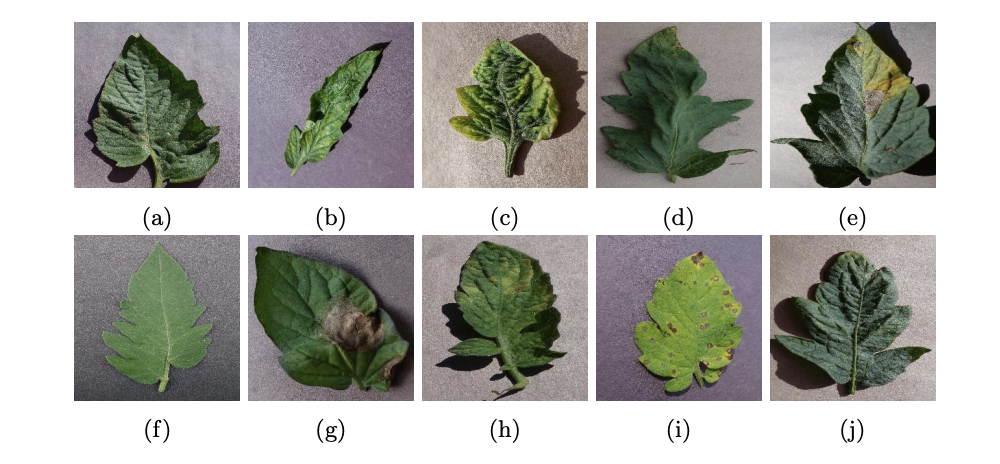
\includegraphics[width=0.8\textwidth]{plant_village_demo} % Replace with your image file
	\caption{A visualization of all tomato leaf image types in the PlantVillage dataset. The following types are contained in the dataset: Target spot (a), Mosaic virus (b), Yellow leaf curl virus (c), Bacterial spot (d), Early bligh (e), Healthy (f), Late blight (g), Leaf mold (h), Septoria leaf spot (i), and Spider mites (j).}
	\label{fig:plantvillage_types}
\end{figure}

\section{Preprocessing}
Each training image was preprocessed using grayscale conversion, histogram
equalization, median filtering, Otsu thresholding, and background subtraction.
Preprocessing enhanced the images to improve the effectiveness and accuracy
of subsequent feature extraction and model training.

\subsection{Grayscale conversion}
The original RGB images were converted to grayscale. We need to do this step because our features are derived from Haralick texture statistics, specifically the GLCM, which requires grayscale input. Diseased leaves have surface texture variations, while healthy leaves are mostly uniform, making texture18 based features appropriate for leaf disease detection. See \ref{fig:rgb_vs_gray} which compares the original RGB image to its grayscale form

\begin{figure}[htbp]
	\centering
	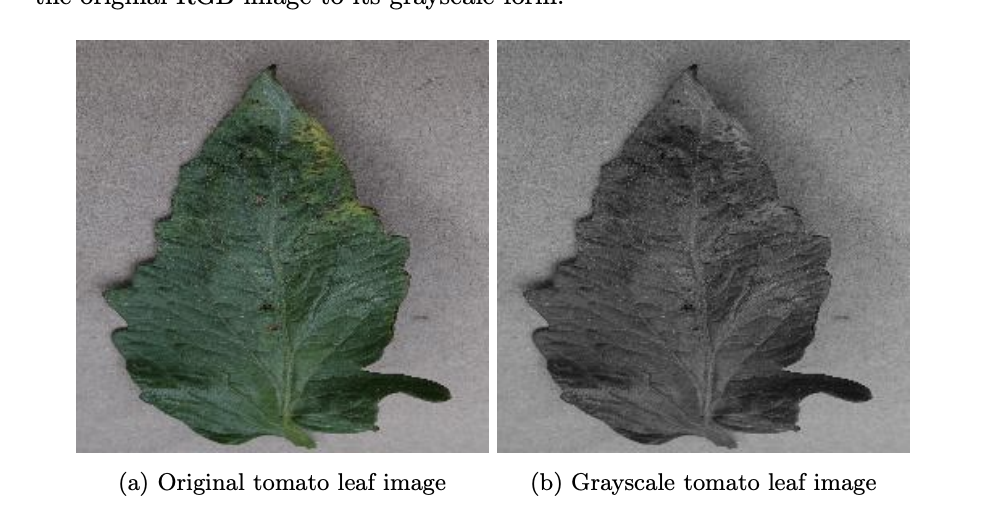
\includegraphics[width=0.8\textwidth]{rgb_demo} % Replace with your image file
	\caption{RGB to grayscale image comparison}
	\label{fig:rgb_vs_gray}
\end{figure}

\subsection{Histogram equalization}
Leaf images in the Plant Village dataset are captured under a variety of
lighting conditions, which complicates segmentation. In bright light, the background can become illuminated and may appear to be a part of the leaf, making
global thresholding methods ineffective. In our experiment, we selected Otsu
segmentation for its simplicity and computational efficiency. This method of
segmentation separates the foreground from the background by maximizing interclass variance, and works best when the image histogram is bimodal. However, uneven lighting typically results in unimodal or irregular histograms, so
segmentation becomes unreliable. By equalizing the histogram of the grayscale
image, the image’s intensity distribution becomes more uniform and closer to
bimodal, which enhances contrast between the foreground and background as
shown in figure \ref{fig:histogram_equalization_demo}. Effectively, histogram equalization improves the performance of subsequent segmentation.

\begin{figure}[htbp]
	\centering
	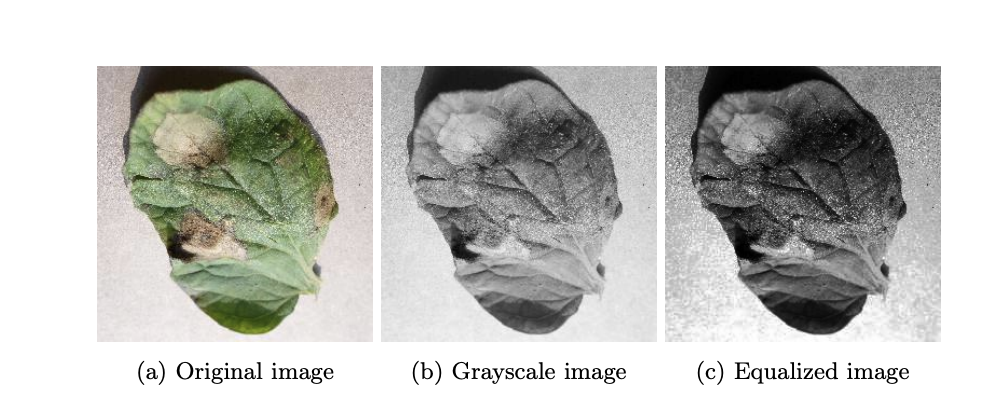
\includegraphics[width=0.8\textwidth]{histogram_equalization_demo} % Replace with your image file
	\caption{Side by side comparison of images showing the contrast enhancement	effect of our histogram equalization step.}
	\label{fig:histogram_equalization_demo}
\end{figure}

\subsection{Median Filtering}
Median filtering is applied to the equalized grayscale image to reduce noise.
Noise can introduce sharp intensity changes and these abrupt variations can
cause parts of the image to be incorrectly classified as part of background rather
than part of the leaf when using global thresholding methods. This will reduce
the overall effectiveness of our segmentation, so we apply median filtering.

% Figure 4.4: Median Filtering
\begin{figure}[htbp]
	\centering
	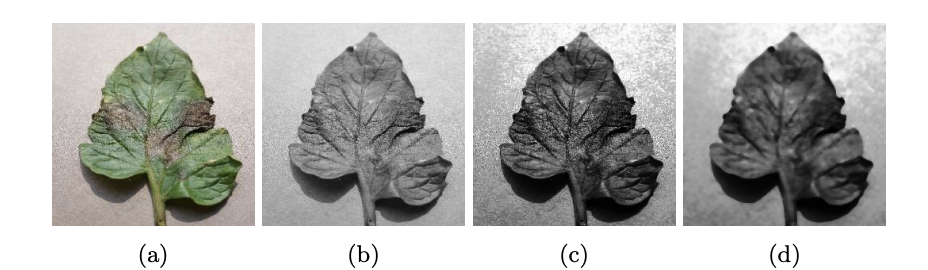
\includegraphics[width=0.8\textwidth]{median_filtering_demo} % Replace with your image file
	\caption{Application of median filtering in our experiment. (a) original image, (b) grayscale image, (c) histogram equalized grayscale image, and (d) median filtered equalized grayscale image.}
	\label{fig:median_filtering_demo}
\end{figure}

\subsection{Segmentation}
In our segmentation step, we apply Otsu thresholding to the median-filtered
image to produce a binary mask. Using this binary mask, background subtraction is then performed on the grayscale image to segment the leaf from the background as figure \ref{fig:segmentation_demo} shows. Our implementation assumes that the background and foreground have sufficient contrast. That is the median-filtered image has a bimodal or near-bimodal histogram distribution. Although the PlantVillage dataset contains images captured under varying conditions, the lighting was
generally uniform, making this assumption reasonable. However, this segmentation method may not generalize well to field environments or poorly lit conditions. Despite this, Otsu’s method is simple to implement and computationally efficient, since one of the goals of our research is developing a cost-effective solution for low-cost greenhouse environments, this trade-off in field-applicability for economicity is acceptable.

% Figure 4.5: Preprocessing Phases
\begin{figure}[htbp]
	\centering
	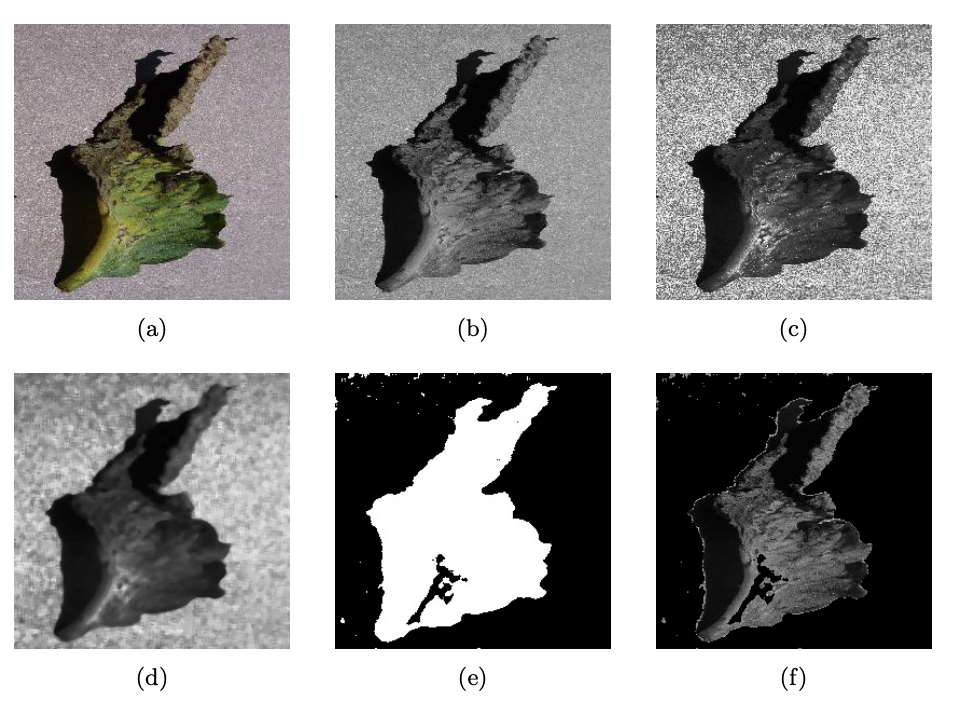
\includegraphics[width=0.8\textwidth]{segmentation_demo} % Replace with your image file
	\caption{A leaf image going through all phases of preprocessing, and concluding with segmentation: (a) original image, (b) grayscale image, (c) histogram equalized grayscale image, (d) median filtered equalized grayscale image, (e) Otsu binary mark, and (f) segmented image.}
	\label{fig:segmentation_demo}
\end{figure}

\clearpage

\subsection{Feature Extraction}
After image segmentation, the GLCM matrix is computed from the segmented
grayscale image, considering only the gray levels corresponding to the leaf.
Should we consider all gray levels, then the quality of our features will be affected
and consequently our classifier’s performance will suffer. Therefore, the accuracy of the segmentation directly influences the quality of the extracted features.
So, we assume that all regions excluded from the segmented image are non-plant
areas. That is gray levels of value 0 are ignored. Without this assumption, the
GLCM is a matrix $P(i, j, \theta, d)$, representing the probability that gray levels $i$
and $j$ occur at an angle $\theta$ and distance $d$ away from each each other. But with $0$
gray levels ignored, then the GLCM represents $P(i, j, \theta, d | \text{part of leaf})$. That
is the GLCM gives us leaf textural information and not background texture metrics.

\paragraph{}
The GLCM matrix requires a choice of distance $d$ and angle $\theta$ for its computation. Higher values of $d$ are more computationally efficient, but give less spatial
textural information. Since we do not use any color information for features,
high $d$ values may lead to less accurate predictions as our model will be trained
with lower textural resolution data. So, we select $1$ as our value for $d$. As for
the angles, we computed the matrix for $0^\circ$, $45^\circ$, $90^\circ$◦ and $135^\circ$. By calculating
the GLCM for multiple angles we get textural information in many different
directions. These 4 angles are sufficient since computing the GLCM for angles
like $180^\circ$, $225^\circ$, $270^\circ$ and $315^\circ$ is essentially just the transpose of GLCMs for $0^\circ$, $45^\circ$, $90^\circ$ and $135^\circ$.

\paragraph{}
For each GLCM obtained from a distance $d$ and angle $\theta$ we calculate several
harlick features from it. Namely as mentioned in the methodology section these
metrics are: energy, contrast, homogeneity, correlation, entropy, angular second
moment, dissimilarity, mean, variance, standard deviation, and homogeneity.
Since, there are $10$ metrics and $4$ angles, we compute $40$ features for each image.
Each feature vector is labelled as healthy or diseased depending on if it was
obtained from a healthy leaf image or a diseased leaf image.

\subsection{Dataset Distribution \& Split}
The PlantVillage dataset is very imbalanced and biased towards images of
diseased leaves. Less than $10\%$ of the tomato leaf images
are labelled healthy. This means that a model trained on this data, will be
biased towards images of diseased leaves and struggle to differentiate between
healthy and non-healthy leaf images. Therefore, the chance of false positives
may be greater. In the context of precision agriculture where the minimization
of pesticide application is desired, a biased model like this could be costly and
undesirable should agriculture decisions be based off the models predictions.
Therefore, in choosing dataset split for training and test data, we ensured that
the overall distributions of diseased and healthy leaves remained the same, so
that our classifier would have greater chances of generalizing well to unseen data.
Specifically we used $90\%$ of the PlantVillage tomato leaf data subset as training
data, and $10\%$ we held out for testing. For model evaluation, we opted for
stratified $10$-fold cross evaluation since the dataset is imbalanced. Essentially,
the split is stratified to preserve the class distributions and mitigate bias to
prevent overfitting.

\subsection{SVM Classifier Training}
We have selected an SVM as our classification mechanism. That is we have
trained a binary classifier that takes in as input harlick texture feature vectors
from the GLCM of a segmented leaf image, and outputs whether or not the
feature belongs to a healthy leaf or diseased tomato leaf.

\paragraph{}
We did not perform an extensive search and comparison to select our hyperparameters, but instead used the radial basis kernel for the SVM which, as
mentioned in the literature review, has performed well and has shown good generalization capabilities in leaf disease detection studies. Additionally, we use
the weighted SVM variant since our dataset is imbalanced so that healthy leaf
images are given more consideration since they are in the minority. This helps
to reduce the risk of overfitting. Once the hyperparameters were fixed, we then
trained and had the model fit the training data.

\section{Model Evaluation}
The results of our experiment are presented below. The tables in \ref{table:svm_performance_test} and \ref{table:svm_performance}
show the performance of our model on the training and data set. We can that
for the training and test data that our model achieved $83\%$ and $84\%$ accuracy
respectively. However this not a good measure of the overall effectiveness and
performance of our model. In fact accuracy on its own is a flawed measure. If
the model were only trained on $99\%$ of leaf images, and $1\%$ of healthy leaves
then it could predict that all images are of diseased leaves and achieve $99\%$
accuracy. But as it is exposed to more unseen data it may not generalize well
and its accuracy in real terms would be much poorer. Therefore, we also examine
the precision, recall and f1-score of our classifier.

\subparagraph{}
Taking a look at the tables we see that recall is $84\%$. Recasting recall in
probabilistic terms, it measures the probability that our classifier will classify a
feature vector as a diseased if the feature is from a diseased leaf image. Let
us denote this as $P(T | D$) where $T$ is the event that the classifier classifies a
feature as diseased, and D is the event that the feature is really from a diseased
leaf image. It is then the case that $P(T | D) = 1 - $ $P(F | D)$, so the probability
that our classifier gives a false negative is only $16\%$ on the training data, so our
models capacity to rule out tomato leaf diseases is good. Our model performed
similarly on the test data. The relative portions of false negatives and true
positives in the confusion matrices \ref{fig:confison_matrix_training_data} and \ref{fig:confison_matrix_test_data} also confirm this claim.

\subparagraph{}
As for precision our model achieved $97\%$ on the training data, and $97\%$ on the
test data. This suggests our model even on unseen data is able to predict that a
leaf image has a disease. On the other hand our dataset was imbalanced, so this
metric is not very good on its own. However, the f1 scores for on the training
data and test data is $90\%$. This high value is because recall and precision are
quite close to one another, suggesting our classifier has a good balance of low
false negatives and accurate predictions. This is further supported by the ROC
and AUC digrams in \ref{fig: ROC & AUC test data} and \ref{fig: ROC & AUC training data}.

\subparagraph{}
The ROC curve in \ref{fig: ROC & AUC training data} shows that our our model on the training data strikes a
good balance between the recall and the false positive rate. The ROC measures
an implicit variable, in the sense that if $P(DiseasedImage$) is the probability
that an image is for a diseased leaf image, if we pick a bound $B$ and classify any
image as diseased if $P(DiseasedImage) > B$, then we get a False positive rate
and true positive rate (Recall) which are plotted as points, and form the ROC.
Taking many different values of $B$ we get the resulting curve. Overall, the curve
deviates from the identify ROC through the origin meaning it is more likely to
give meaningful predictions. The ROC curve \ref{fig: ROC & AUC test data} is similar to the training data
ROC, and so this suggests our SVM classifier generalizes well to the unseen test
data. Furthermore, the AUC (area under the curve) in both figures is close to
$1$ at least$0.90$ for both. An AUC of $1$ is what a perfect classifer would achieve,
so our classifier in terms of this metric performs well in detecting tomato leaf
diseases.

\begin{table}[htbp]
	\centering
	\begin{tabular}{|l|l|l|l|l|}
		\hline
		\textbf{Dataset size} & \textbf{Accuracy} & \textbf{Precision} & \textbf{Recall} & \textbf{F1} \\ \hline
		14409 images          & 83\%             & 97\%              & 84\%           & 90\%        \\ \hline
	\end{tabular}
	\caption{Summary of our SVM classifier’s average performance on the training data running after 10-fold stratified cross validation.}
	\label{table:svm_performance}
\end{table}

\begin{table}[htbp]
	\centering
	\begin{tabular}{|l|l|l|l|l|}
		\hline
		\textbf{Dataset size} & \textbf{Accuracy} & \textbf{Precision} & \textbf{Recall} & \textbf{F1} \\ \hline
		1602 images          & 84\%             & 97\%              & 84\%           & 90\%        \\ \hline
	\end{tabular}
	\caption{ Summary of our SVM classifier’s performance on the the test data.}
	\label{table:svm_performance_test}
\end{table}

\begin{figure}[htbp]
	\centering
	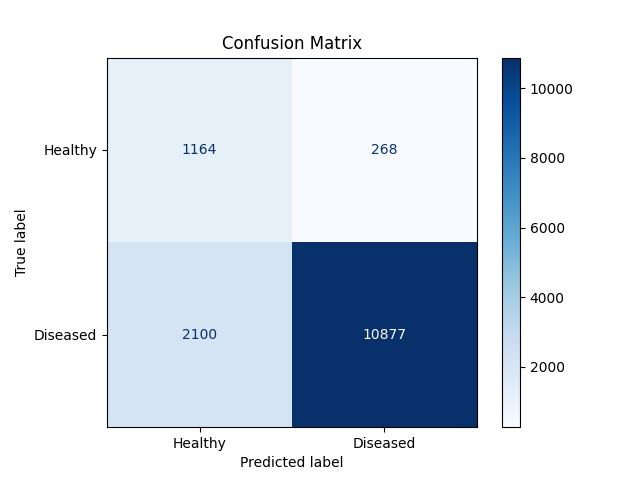
\includegraphics[width=0.8\textwidth]{confusion_matrix_training.png} % Replace with your image file
	\caption{Confusion matrix for our model's prediction on the training data}
	\label{fig:confison_matrix_training_data}
\end{figure}

\begin{figure}[htbp]
	\centering
	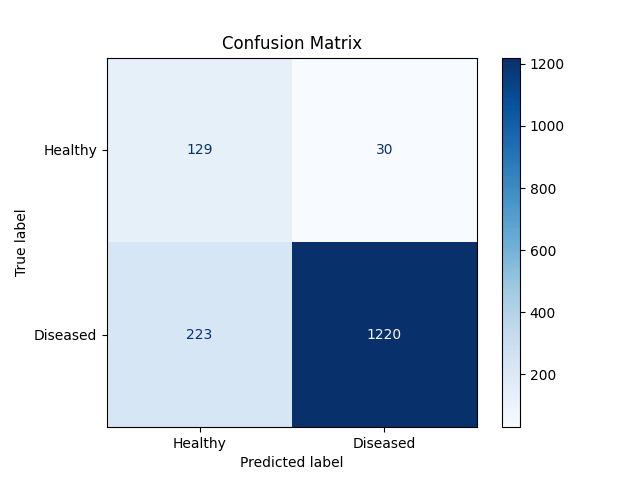
\includegraphics[width=0.8\textwidth]{confusion_matrix_test.png} % Replace with your image file
	\caption{Confusion matrix for our model's prediction on the test data}
	\label{fig:confison_matrix_test_data}
\end{figure}

\begin{figure}[htbp]
	\centering
	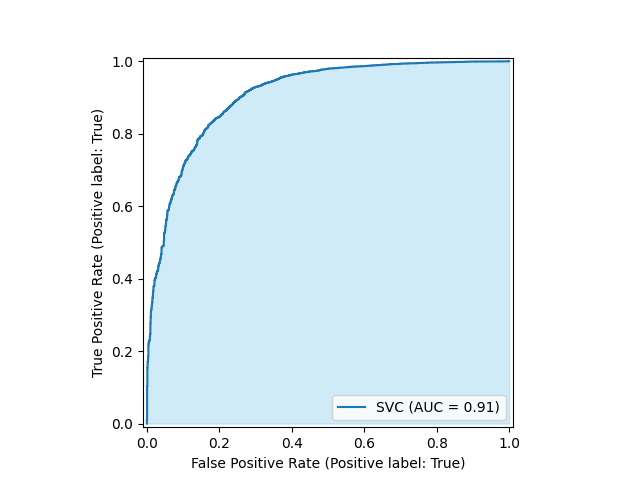
\includegraphics[width=0.8\textwidth]{ROC_and_AUC_training.png} % Replace with your image file
	\caption{ROC and AUC for our model on the training data aftet 10 fold stratified cross validation.}
	\label{fig: ROC & AUC training data}
\end{figure}

\begin{figure}[htbp]
	\centering
	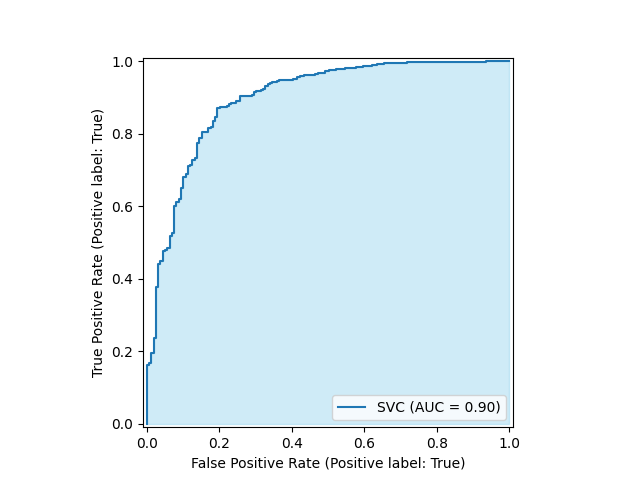
\includegraphics[width=0.8\textwidth]{ROC_AUC_Test_Data.png} % Replace with your image file
	\caption{ROC and AUC for our model after predictions on the test data.}
	\label{fig: ROC & AUC test data}
\end{figure}

\clearpage

\section{Limitations}
As mentioned earlier, the PlantVillage dataset is imbalanced, and only contains less than $10\%$ of healthy tomato leaf images. The confusion matrix 4.7
shows that our classifier struggles to differentiate between diseased and healthy
leaf images. Even though, we reduced the bias by performing stratified test-training data split. This suggests to really be sure of the generalizability of our
solutions, we need to evaluate the performance of classification on a balanced
data set, or on data with a different distribution than PlantVillage.

\subparagraph{}
Also, in developing an economical solution we made a trade-off in terms of
segmentation methods. Opting for simple low complexity segmentation like
Otsu thresholding is more computationally efficient, but it struggles with images
taken with uneven lighting. Therefore, the overall accuracy of feature vectors
and predictions may be compromised by cheaper segmentation choices. On the
other hand, machine learning and deep learning segmentation methods are more
robust, but may be prohibitive in resource constrained contexts.

\subparagraph{}
Additionally, textural feature vectors computed from the GLCM can be computationally expensive depending on the size of the image, and the number of
gray levels. In our research we used 256x256 8-bit images, so on modern hardware these calculations are not particularly painful, but in practice these images
may be substantially larger and then other considerations like quantization or
binning of gray level values may need to be done to practically use our solution

\chapter{Conclusion}

This research set out to build an accessible open-source tool for detecting
tomato leaf diseases in low-cost greenhouse settings. By leveraging modular
computer vision libraries and large public datasets like PlantVillage, we developed an economical SVM classifier that achieved strong accuracy and F1 scores
on its training and test data. This work extends existing literature by showing
the applicability, generalizability, and effectiveness of SVM classifiers for tomato
leaf disease detection. Despite challenges with dataset imbalance and the limits
of Otsu segmentation in poor lighting conditions, our solution remains practical for greenhouse use and can be easily verified, extended, or modified. Most
importantly, this project shows that efficient and adaptable disease detection
is possible with open-source tools. Reproducible, shareable, and modular approaches mean plant phenotyping does not have to be reserved for those with
large capital or proprietary software. In future, this method can be turned into
a mobile application, making tomato leaf disease detection more accessible to
growers and communities everywhere.